% -----------------------------------------------------------------------------
% flow-chart.tex --- Standalone TikZ source for the Tethys workflow figure
% used in main_v4.tex (Figure 2).
%
% Compile to flow-chart.pdf with:
%     pdflatex flow-chart.tex
% (twice if the PDF box is mis-sized on the first pass).
%
% The standalone class crops the output to the bounding box of the picture
% so the resulting PDF has no page margins, which lets us include it via
%     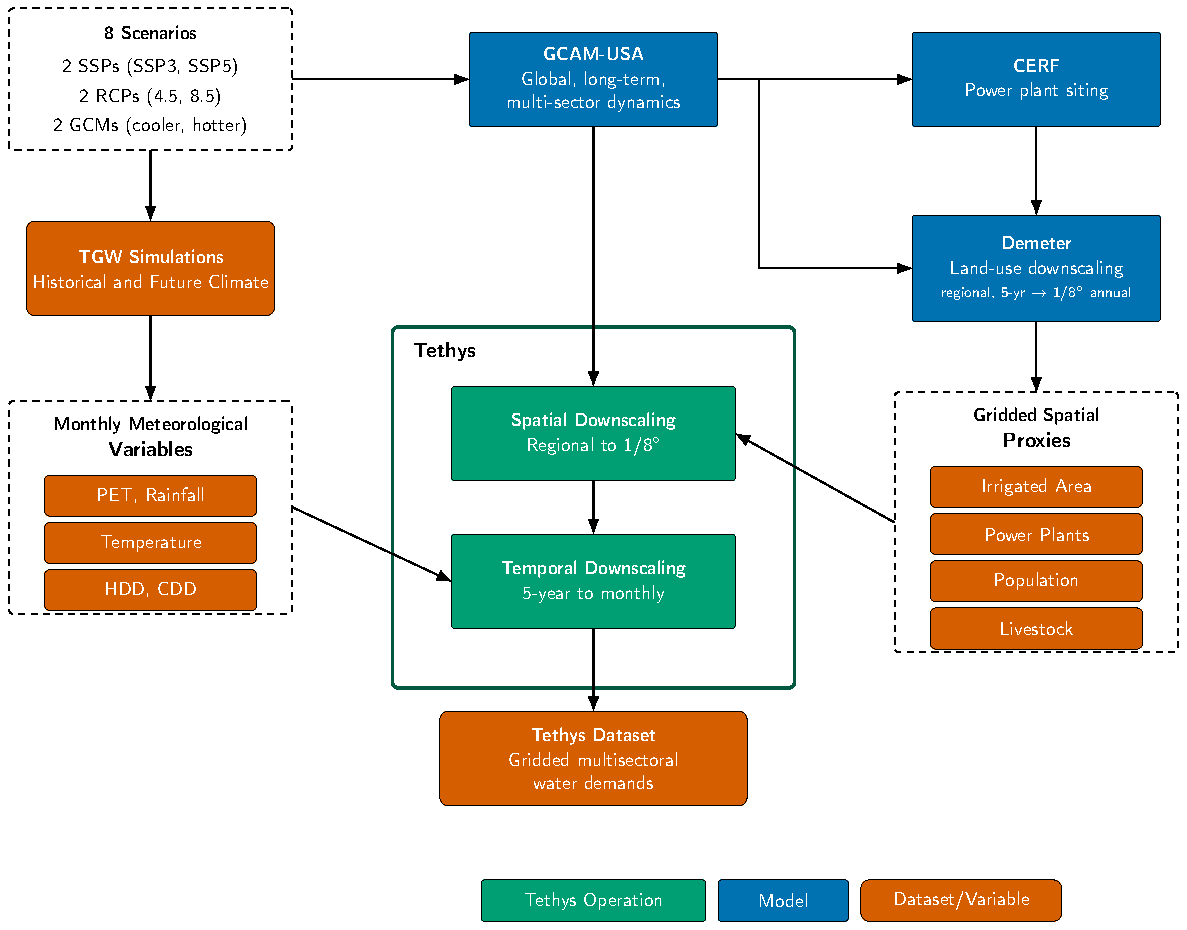
\includegraphics[width=\textwidth]{flow-chart.pdf}
% in main_v4.tex without scaling artifacts.
%
% Colorblind-safe palette (Okabe-Ito 2008; Wong, Nature Methods 2011, 8:441),
% matching the dominant-sector map in Figure 1. White background.
% -----------------------------------------------------------------------------
\documentclass[tikz,border=4pt]{standalone}
%\usepackage[T1]{fontenc}
\usepackage{tikz}
\usetikzlibrary{positioning, arrows.meta, fit, backgrounds, shapes.geometric}

\definecolor{modelfill}{HTML}{0072B2}    % blue: data-providing models
\definecolor{opfill}{HTML}{009E73}       % bluish green: Tethys operations
\definecolor{datafill}{HTML}{D55E00}     % vermillion: datasets / variables
\definecolor{tethysrule}{HTML}{005840}   % darker green for the Tethys outline

\begin{document}
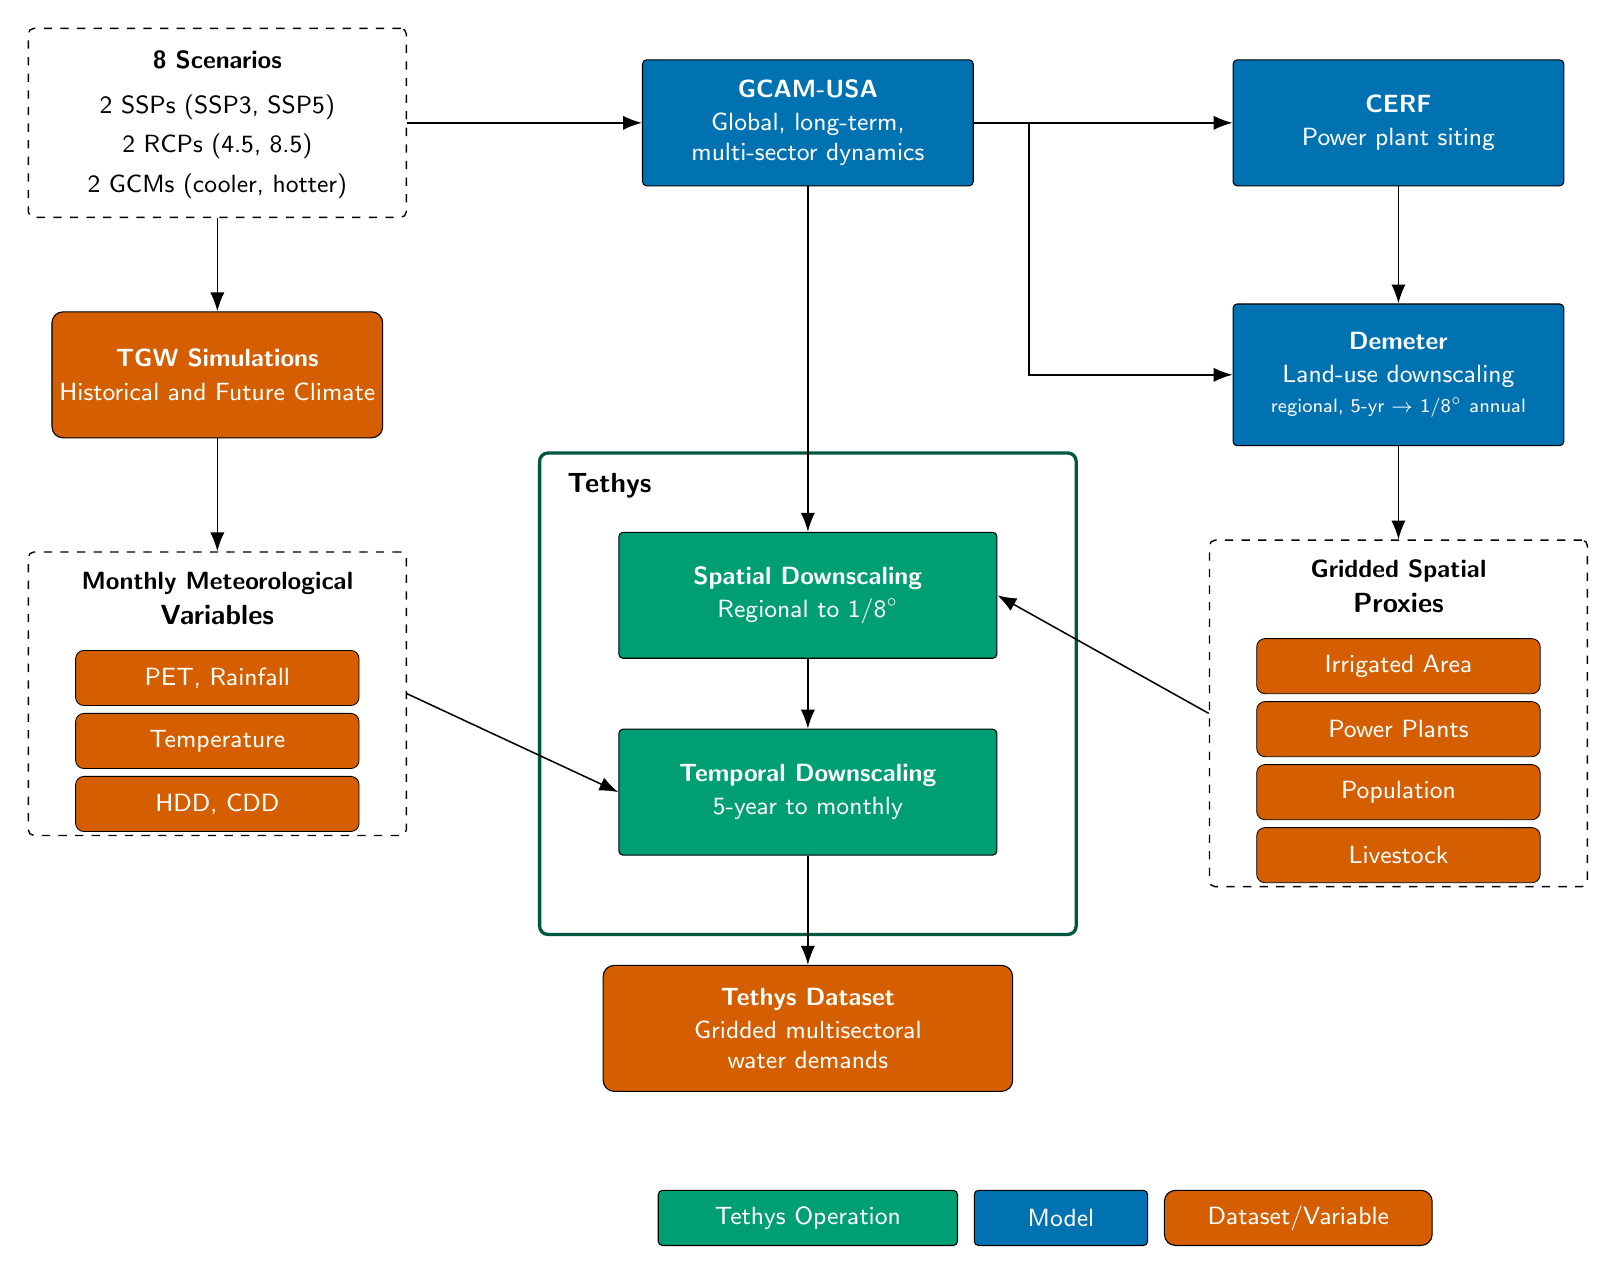
\begin{tikzpicture}[
  font=\sffamily\small,
  every node/.style={align=center, %font=\ssfamily\small, 
  text=white},
  model/.style={
    rectangle, draw=black, line width=0.4pt,
    fill=modelfill,
    rounded corners=1.5pt,
    minimum width=42mm, minimum height=16mm,
    inner sep=2pt
  },
  op/.style={
    rectangle, draw=black, line width=0.4pt,
    fill=opfill,
    rounded corners=1.5pt,
    minimum width=48mm, minimum height=16mm,
    inner sep=2pt
  },
  data/.style={
    rectangle, draw=black, line width=0.4pt,
    fill=datafill,
    rounded corners=4pt,
    minimum width=42mm, minimum height=12mm,
    inner sep=2pt
  },
  smalldata/.style={
    rectangle, draw=black, line width=0.3pt,
    fill=datafill,
    rounded corners=3pt,
    minimum width=36mm, minimum height=7mm,
    inner sep=1pt
  },
  groupbox/.style={
    rectangle, draw=black, line width=0.5pt, dashed,
    rounded corners=2pt,
    inner sep=4pt,
    fill=none,
    text=black
  },
  tethysbox/.style={
    rectangle, draw=tethysrule, line width=1.2pt,
    rounded corners=3pt,
    inner sep=10mm,
    fill=none,
    text=black
  },
  arrow/.style={-{Latex[length=2.4mm]}, line width=0.55pt, color=black},
  bglabel/.style={font=\sffamily\bfseries\small, text=black, align=center}
]

% =============================================================================
% Absolute coordinate grid (units = cm). Columns at x = -7.5 / 0 / +7.5.
% Rows are far enough apart that no node overlaps any other node and there is
% room for the Tethys wrapper outline around (spatial, temporal).
% =============================================================================

% --- Row 0 (top): Scenarios | GCAM-USA | CERF
\node[groupbox, minimum width=48mm, minimum height=24mm] (scenariobox) at (-7.5, 0) {};
\node[bglabel] at ([yshift=8mm]scenariobox.center) {\textbf{8 Scenarios}};
\node[bglabel, font=\sffamily\small] at ([yshift=2mm]scenariobox.center) {2 SSPs (SSP3, SSP5)};
\node[bglabel, font=\sffamily\small] at ([yshift=-3mm]scenariobox.center) {2 RCPs (4.5, 8.5)};
\node[bglabel, font=\sffamily\small] at ([yshift=-8mm]scenariobox.center) {2 GCMs (cooler, hotter)};

\node[model] (gcam) at (0, 0) {%
  \textbf{GCAM-USA}\\[1pt]
  Global, long-term,\\multi-sector dynamics
};
\node[model] (cerf) at (7.5, 0) {%
  \textbf{CERF}\\[1pt]
  Power plant siting
};

% --- Row 1: TGW Simulations | (gap) | Demeter
\node[data, minimum height=16mm] (tgw) at (-7.5, -3.2) {%
  \textbf{TGW Simulations}\\[1pt]
  Historical and Future Climate
};
\node[model, minimum height=18mm] (demeter) at (7.5, -3.2) {%
  \textbf{Demeter}\\[1pt]
  Land-use downscaling\\
  \scriptsize regional, 5-yr $\to$ 1/8$^{\circ}$ annual
};

% --- Row 2: Spatial Downscaling at center
\node[op] (spatial) at (0, -6.0) {%
  \textbf{Spatial Downscaling}\\[1pt]
  Regional to 1/8$^{\circ}$
};

% --- Row 3: Temporal Downscaling
\node[op] (temporal) at (0, -8.5) {%
  \textbf{Temporal Downscaling}\\[1pt]
  5-year to monthly
};

% --- Tethys wrapper around spatial + temporal (no fill, just a thick outline)
\begin{scope}[on background layer]
  \node[tethysbox, fit=(spatial)(temporal)] (tethys) {};
\end{scope}
\node[bglabel, anchor=north west, font=\sffamily\bfseries]
     at ([xshift=2.5mm, yshift=-1.5mm]tethys.north west) {Tethys};

% --- Met-vars and proxies groupboxes flank Tethys
\node[groupbox, minimum width=48mm, minimum height=36mm] (metbox) at (-7.5, -7.25) {};
\node[bglabel] at ([yshift=14mm]metbox.center) {\textbf{Monthly Meteorological}};
\node[bglabel, font=\sffamily\bfseries] at ([yshift=10mm]metbox.center) {\textbf{Variables}};
\node[smalldata] (m1) at ([yshift=2mm]metbox.center) {PET, Rainfall};
\node[smalldata] (m2) at ([yshift=-6mm]metbox.center) {Temperature};
\node[smalldata] (m3) at ([yshift=-14mm]metbox.center) {HDD, CDD};

\node[groupbox, minimum width=48mm, minimum height=44mm] (proxybox) at (7.5, -7.5) {};
\node[bglabel] at ([yshift=18mm]proxybox.center) {\textbf{Gridded Spatial}};
\node[bglabel, font=\sffamily\bfseries] at ([yshift=14mm]proxybox.center) {\textbf{Proxies}};
\node[smalldata] (p1) at ([yshift=6mm]proxybox.center) {Irrigated Area};
\node[smalldata] (p2) at ([yshift=-2mm]proxybox.center) {Power Plants};
\node[smalldata] (p3) at ([yshift=-10mm]proxybox.center) {Population};
\node[smalldata] (p4) at ([yshift=-18mm]proxybox.center) {Livestock};

% --- Row 4: Tethys Dataset (output)
\node[data, minimum width=52mm, minimum height=16mm] (out) at (0, -11.5) {%
  \textbf{Tethys Dataset}\\[1pt]
  Gridded multisectoral\\water demands
};

% =============================================================================
% Arrows
% =============================================================================
\draw[arrow] (scenariobox.east) -- (gcam.west);
\draw[arrow] (gcam.east) -- (cerf.west);
\draw[arrow] (gcam.south) -- (spatial.north);
\draw[arrow] (cerf.south) -- (demeter.north);
\draw[arrow] (gcam.east) -- ++(7mm,0) |- (demeter.west);
\draw[arrow] (scenariobox.south) -- (tgw.north);
\draw[arrow] (tgw.south) -- (metbox.north);
\draw[arrow] (metbox.east) -- (temporal.west);
\draw[arrow] (proxybox.west) -- (spatial.east);
\draw[arrow] (demeter.south) -- (proxybox.north);
\draw[arrow] (spatial.south) -- (temporal.north);
\draw[arrow] (temporal.south) -- (out.north);

% =============================================================================
% Legend (bottom centered, on white)
% =============================================================================
\node[op, minimum width=38mm, minimum height=7mm] (legop)
  at ([yshift=-16mm]out.south) {Tethys Operation};
\node[model, minimum width=22mm, minimum height=7mm, right=2mm of legop] (legmodel) {Model};
\node[data, minimum width=34mm, minimum height=7mm, right=2mm of legmodel] (legdata) {Dataset/Variable};

\end{tikzpicture}
\end{document}
